\documentclass[11pt,a4paper,oneside]{report}
\usepackage{amsmath,amssymb,calc,ifthen}
\usepackage{float}
%\usepackage{cancel}
\usepackage[table,usenames,dvipsnames]{xcolor} % for coloured cells in tables
\usepackage{tikz}
% Allows us to click on links and references!
\usepackage{hyperref}
\usepackage{url}
\hypersetup{
colorlinks,
citecolor=black,
filecolor=black,
linkcolor=black,
urlcolor=black
}
% Nice package for plotting graphs
% See excellent guide:
% http://www.tug.org/TUGboat/tb31-1/tb97wright-pgfplots.pdf
\usetikzlibrary{plotmarks,shapes}
\usepackage{amsmath,graphicx}
\usepackage{epstopdf}
\usepackage{caption}
\usepackage{subcaption}
% highlight - useful for TODOs and similar
\usepackage{color}
\newcommand{\hilight}[1]{\colorbox{yellow}{#1}}
\newcommand\ci{\perp\!\!\!\perp} % perpendicular sign
\newcommand*\rfrac[2]{{}^{#1}\!/_{#2}} % diagonal fraction
\newcommand\SLASH{\char`\\}
\usepackage{listings}
% margin size
\usepackage[margin=0.65in]{geometry}

\usepackage{titlesec} % reduce spacing after subsections

\titlespacing\subsection{0pt}{4pt plus 4pt minus 2pt}{4pt plus 2pt minus 2pt}

\usepackage{multicol}

\tikzstyle{state}=[circle,thick,draw=black, align=center, minimum size=2.1cm,
inner sep=0]
\tikzstyle{vertex}=[circle,thick,draw=black]
\tikzstyle{terminal}=[rectangle,thick,draw=black]
\tikzstyle{edge} = [draw,thick]
\tikzstyle{lo} = [edge,dotted]
\tikzstyle{hi} = [edge]
\tikzstyle{trans} = [edge,->]
\definecolor{mygreen}{rgb}{0,0.6,0}
\definecolor{mygray}{rgb}{0.5,0.5,0.5}
\definecolor{mymauve}{rgb}{0.58,0,0.82}
\DeclareMathOperator*{\argmin}{arg\,min}
\DeclareMathOperator*{\argmax}{arg\,max}
\lstset{ %
backgroundcolor=\color{white}, % choose the background color; you must add
%\usepackage{color} or \usepackage{xcolor}
basicstyle=\footnotesize, % the size of the fonts that are used for the
%code
breakatwhitespace=false, % sets if automatic breaks should only happen
%at whitespace
breaklines=true, % sets automatic line breaking
captionpos=b, % sets the caption-position to bottom
commentstyle=\color{mygreen}, % comment style
deletekeywords={...}, % if you want to delete keywords from the
%given language
escapeinside={\%*}{*)}, % if you want to add LaTeX within your code
extendedchars=true, % lets you use non-ASCII characters; for
%8-bits encodings only, does not work with UTF-8
frame=single, % adds a frame around the code
keepspaces=true, % keeps spaces in text, useful for keeping
%indentation of code (possibly needs columns=flexible)
keywordstyle=\color{blue}, % keyword style
language=Octave, % the language of the code
morekeywords={*,...}, % if you want to add more keywords to the set
numbers=left, % where to put the line-numbers; possible
%values are (none, left, right)
numbersep=5pt, % how far the line-numbers are from the code
numberstyle=\tiny\color{mygray}, % the style that is used for the line-numbers
rulecolor=\color{black}, % if not set, the frame-color may be changed
%on line-breaks within not-black text (e.g. comments (green here))
showspaces=false, % show spaces everywhere adding particular
%underscores; it overrides 'showstringspaces'
showstringspaces=false, % underline spaces within strings only
showtabs=false, % show tabs within strings adding particular
%underscores
stepnumber=2, % the step between two line-numbers. If it's
%1, each line will be numbered
stringstyle=\color{mymauve}, % string literal style
tabsize=2, % sets default tabsize to 2 spaces
title=\lstname % show the filename of files included with
%\lstinputlisting; also try caption instead of title
}
\title{Computational Modelling for Biomedical Imaging - Individual Report}
\author{
Razvan Valentin Marinescu\\
Student Number: 14060166\\
\texttt{razvan.marinescu.14@ucl.ac.uk}
}



\begin{document}
\belowdisplayskip=12pt plus 3pt minus 9pt
\belowdisplayshortskip=7pt plus 3pt minus 4pt
\maketitle{}



\rowcolors{2}{gray!25}{white}

\subsection*{Task 1 - Visual assessment}

\begin{figure}[H]
  \centering
  \begin{subfigure}[b]{0.1\textwidth}
    Reg 1\\\\\\\\
  \end{subfigure}%
  \hspace*{-1.9em}
  \begin{subfigure}[b]{0.3\textwidth}
	  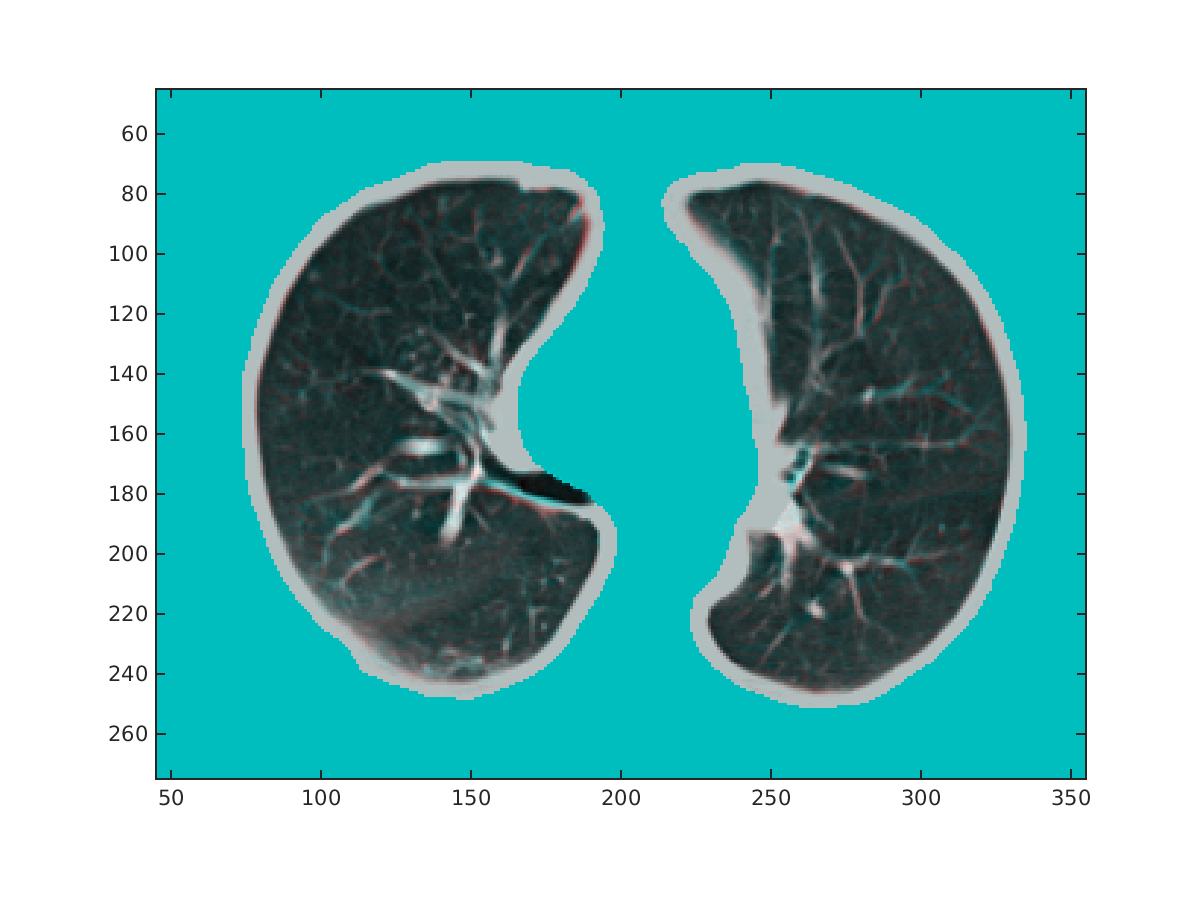
\includegraphics[width=\textwidth, trim=20 20 20 20]{figures/reg1/reg1_1_66.png}
  \end{subfigure}%
%         ~ %add desired spacing between images, e. g. ~, \quad, \qquad, \hfill etc.
    %(or a blank line to force the subfigure onto a new line)
  \begin{subfigure}[b]{0.3\textwidth}
	  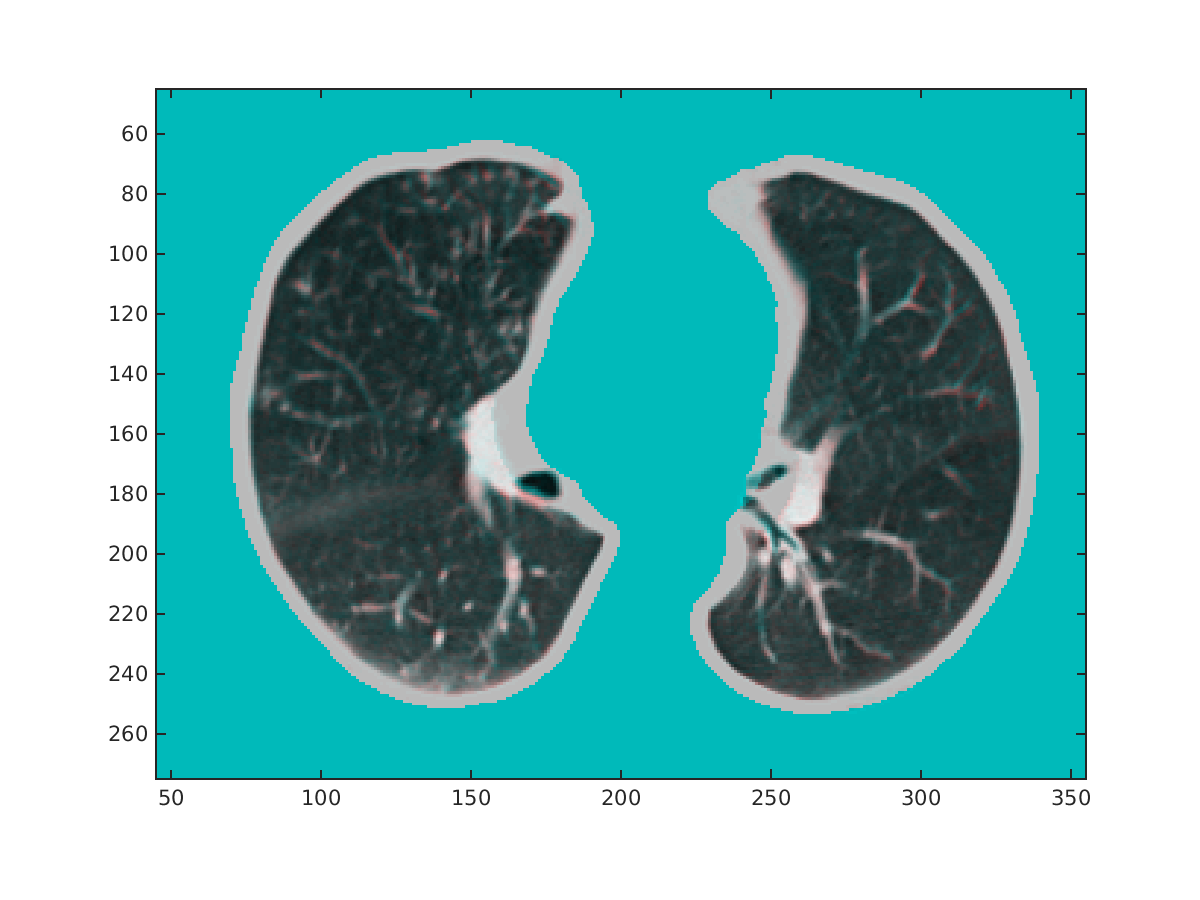
\includegraphics[width=\textwidth, trim=20 20 20 20]{figures/reg1/reg2_5_60.png}
  \end{subfigure}
%         ~ %add desired spacing between images, e. g. ~, \quad, \qquad, \hfill etc.
    %(or a blank line to force the subfigure onto a new line)
  \begin{subfigure}[b]{0.3\textwidth}
	  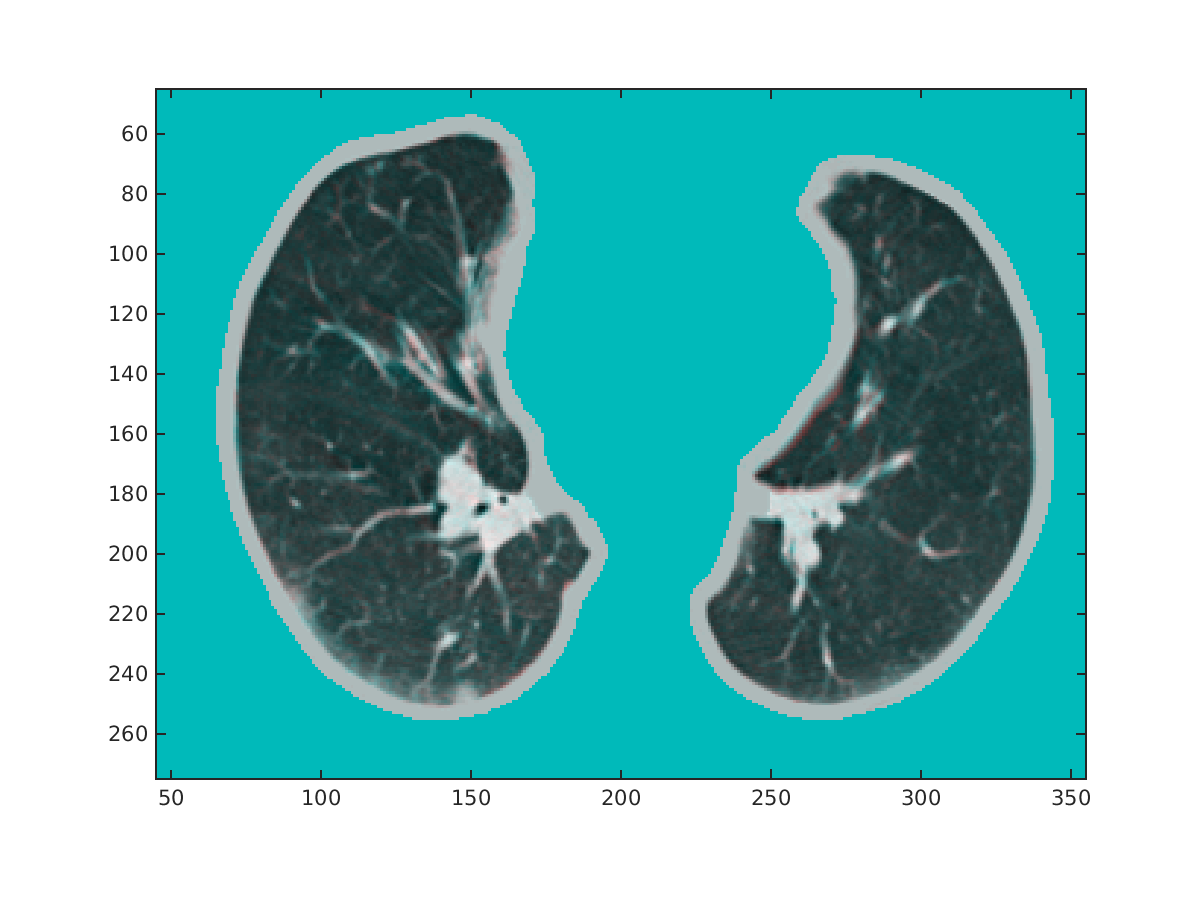
\includegraphics[width=\textwidth, trim=20 20 20 20]{figures/reg1/reg3_2_49.png}
  \end{subfigure}
  
%         ~

  \begin{subfigure}[b]{0.1\textwidth}
    Reg 2\\\\\\\\\\
  \end{subfigure}%
  \hspace*{-1.9em}
  \begin{subfigure}[b]{0.3\textwidth}
	  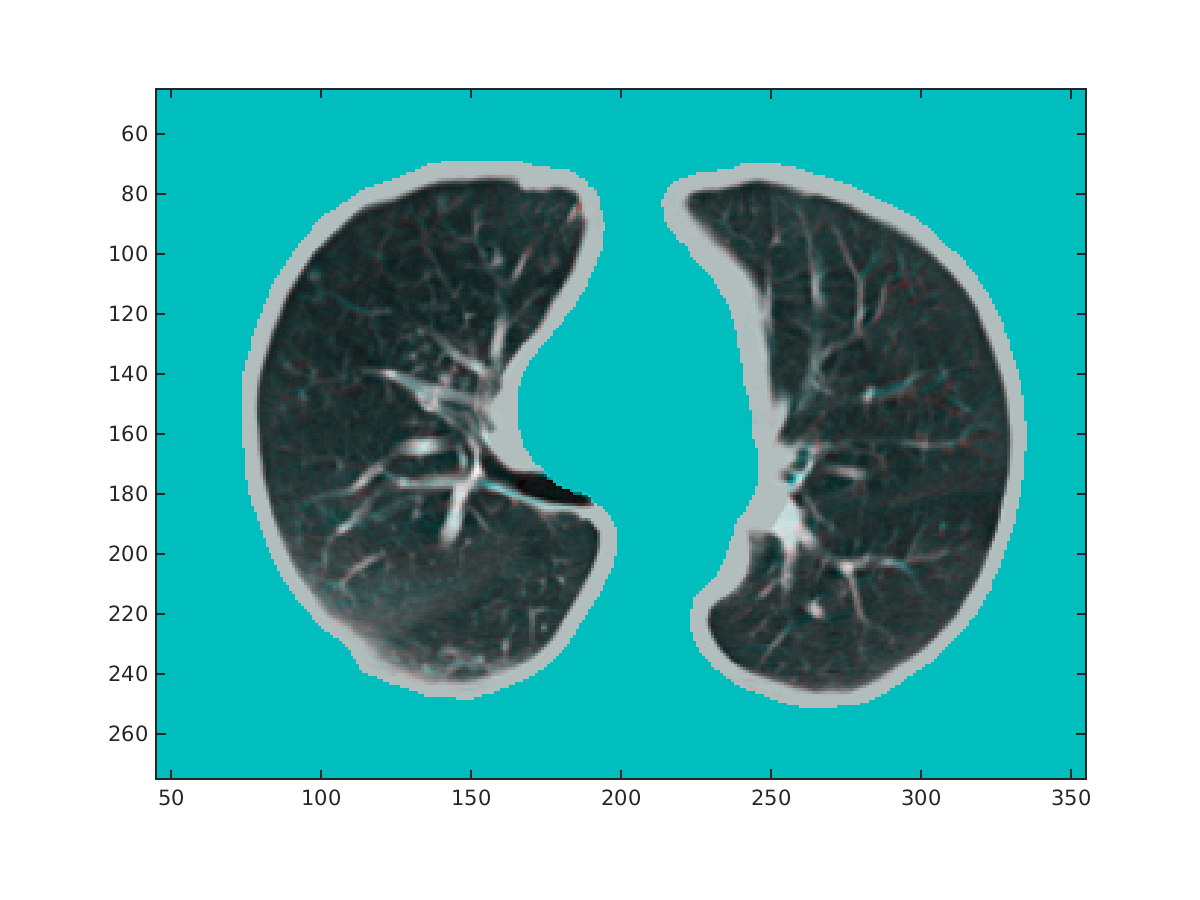
\includegraphics[width=\textwidth, trim=20 20 20 20]{figures/reg2/reg1_1_66.png}
	  \caption{Couch 1, volume 1, slice 66}
	  \label{fig:c11}
  \end{subfigure}%
%         ~ %add desired spacing between images, e. g. ~, \quad, \qquad, \hfill etc.
%           %(or a blank line to force the subfigure onto a new line)
  \begin{subfigure}[b]{0.3\textwidth}
	  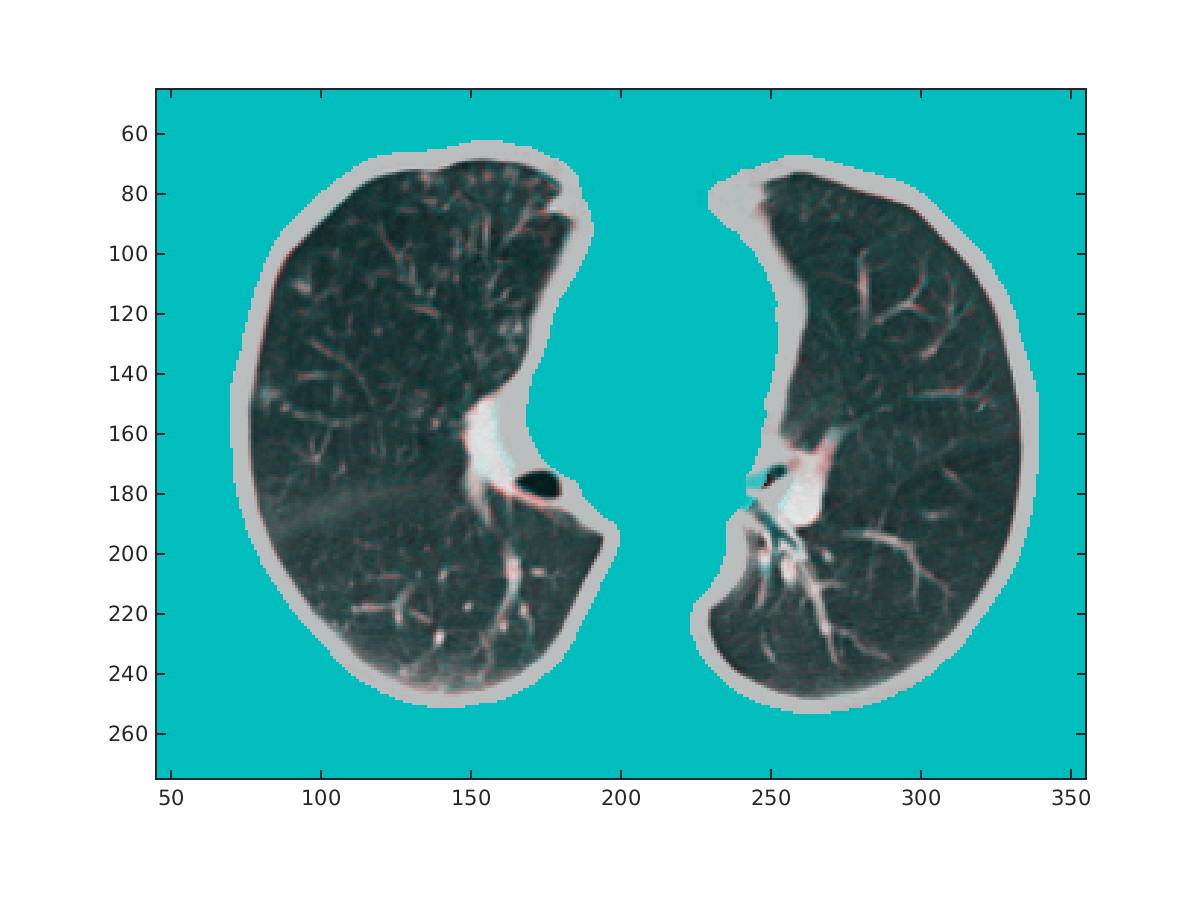
\includegraphics[width=\textwidth, trim=20 20 20 20]{figures/reg2/reg2_5_60.png}
	  \caption{Couch 2, volume 5, slice 60}
	  \label{fig:c12}
  \end{subfigure}
%         ~ %add desired spacing between images, e. g. ~, \quad, \qquad, \hfill etc.
    %(or a blank line to force the subfigure onto a new line)
  \begin{subfigure}[b]{0.3\textwidth}
	  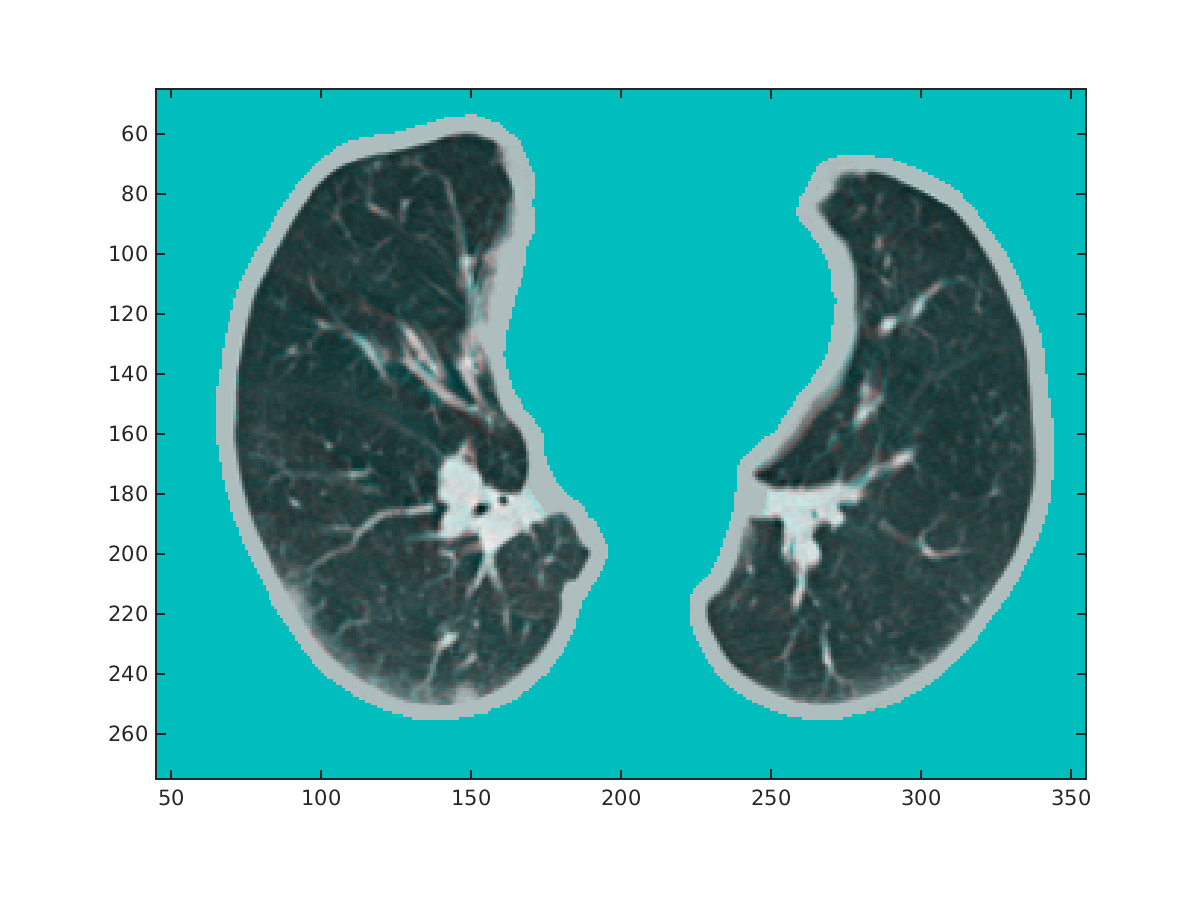
\includegraphics[width=\textwidth, trim=20 20 20 20]{figures/reg2/reg3_2_49.png}
	  \caption{Couch 3, volume 2, slice 49}
	  \label{fig:c13}
  \end{subfigure}
  
  ~
  \vfill
  
  \begin{subfigure}[b]{0.1\textwidth}
    Reg 1\\\\\\\\
  \end{subfigure}%
  \hspace*{-1.9em}
  \begin{subfigure}[b]{0.3\textwidth}
	  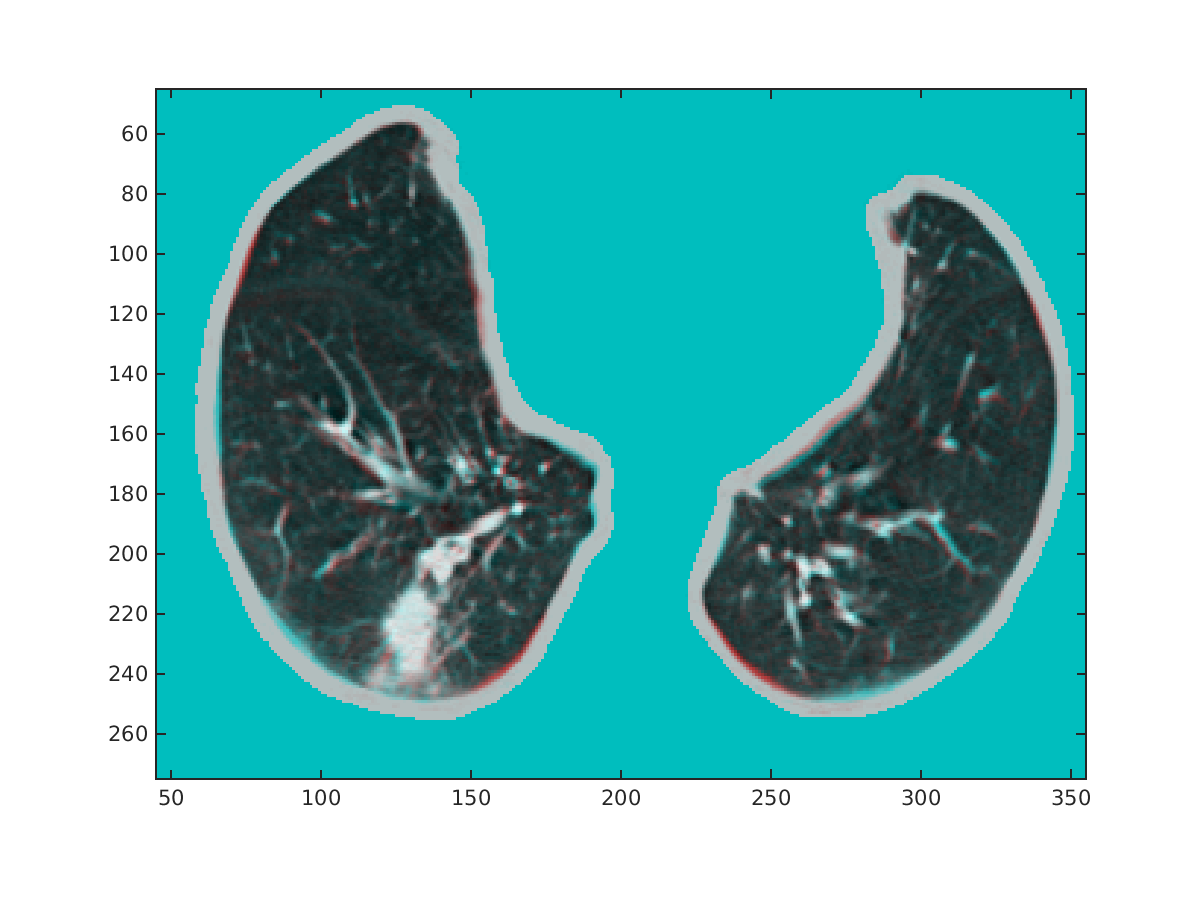
\includegraphics[width=\textwidth, trim=20 20 20 20]{figures/reg1/reg4_8_37.png}
  \end{subfigure}%
%         ~ %add desired spacing between images, e. g. ~, \quad, \qquad, \hfill etc.
    %(or a blank line to force the subfigure onto a new line)
  \begin{subfigure}[b]{0.3\textwidth}
	  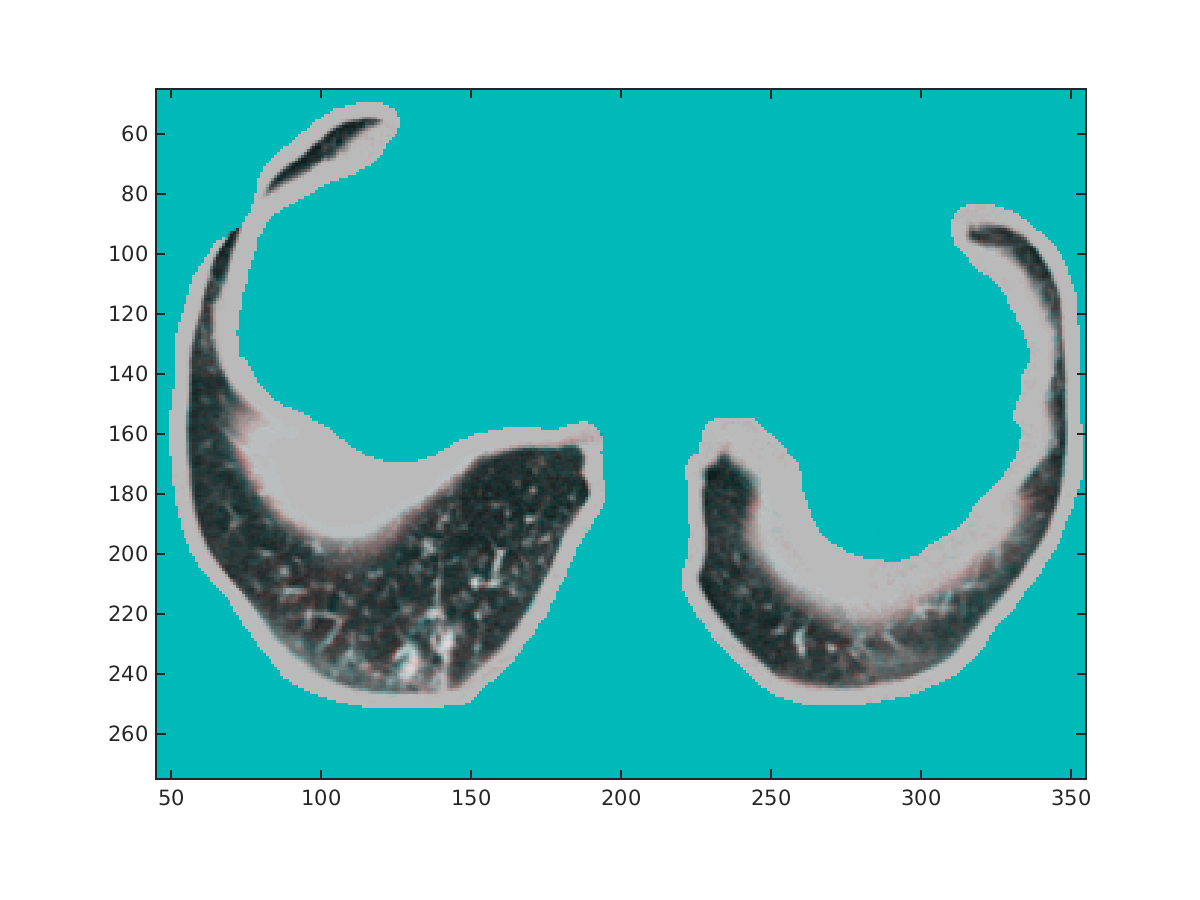
\includegraphics[width=\textwidth, trim=20 20 20 20]{figures/reg1/reg5_4_25.png}
  \end{subfigure}
%         ~ %add desired spacing between images, e. g. ~, \quad, \qquad, \hfill etc.
    %(or a blank line to force the subfigure onto a new line)
  \begin{subfigure}[b]{0.3\textwidth}
	  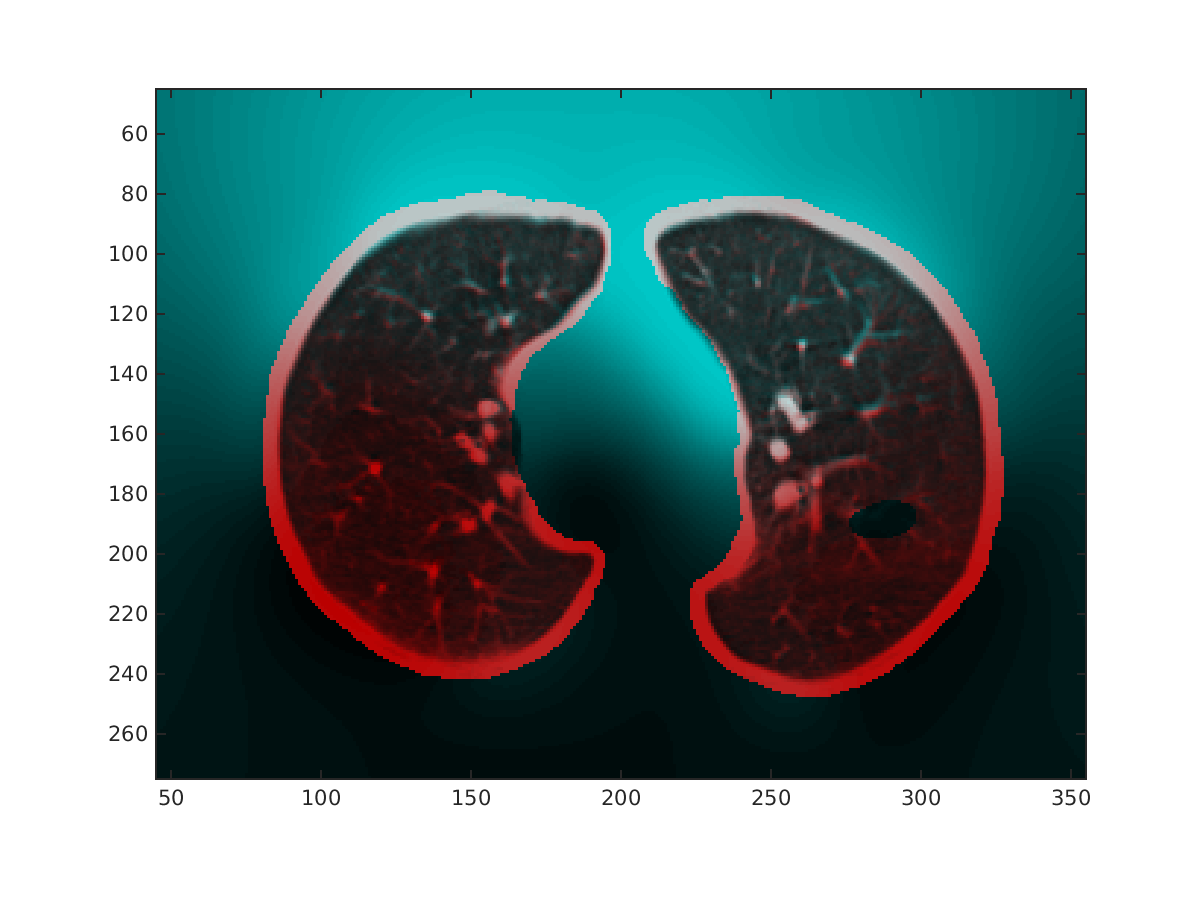
\includegraphics[width=\textwidth, trim=20 20 20 20]{figures/reg1/reg1_6_76.png}
  \end{subfigure}
  
%         ~

  \begin{subfigure}[b]{0.1\textwidth}
    Reg 2\\\\\\\\\\
  \end{subfigure}%
  \hspace*{-1.9em}
  \begin{subfigure}[b]{0.3\textwidth}
	  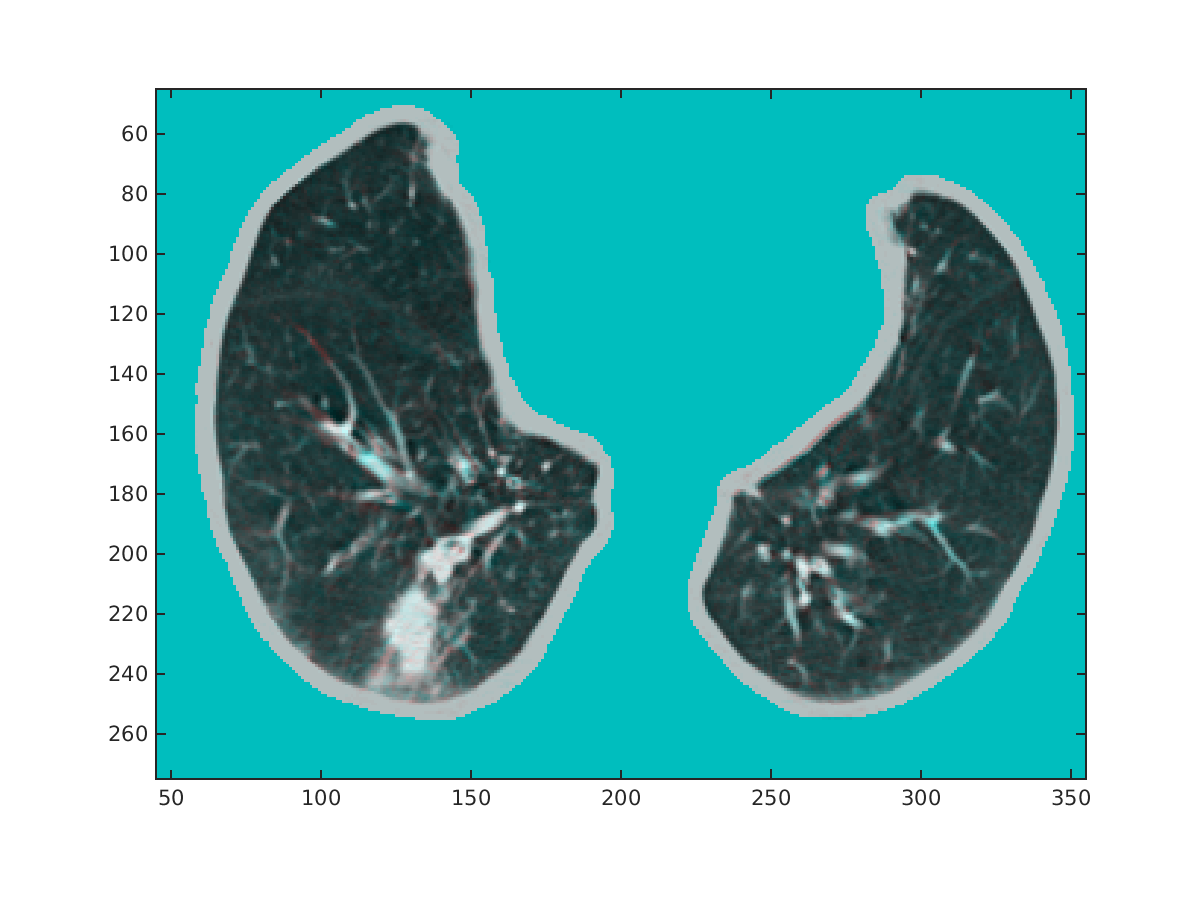
\includegraphics[width=\textwidth, trim=20 20 20 20]{figures/reg2/reg4_8_37.png}
	  \caption{Couch 4, volume 8, slice 37}
	  \label{fig:c21}
  \end{subfigure}%
%         ~ %add desired spacing between images, e. g. ~, \quad, \qquad, \hfill etc.
    %(or a blank line to force the subfigure onto a new line)
  \begin{subfigure}[b]{0.3\textwidth}
	  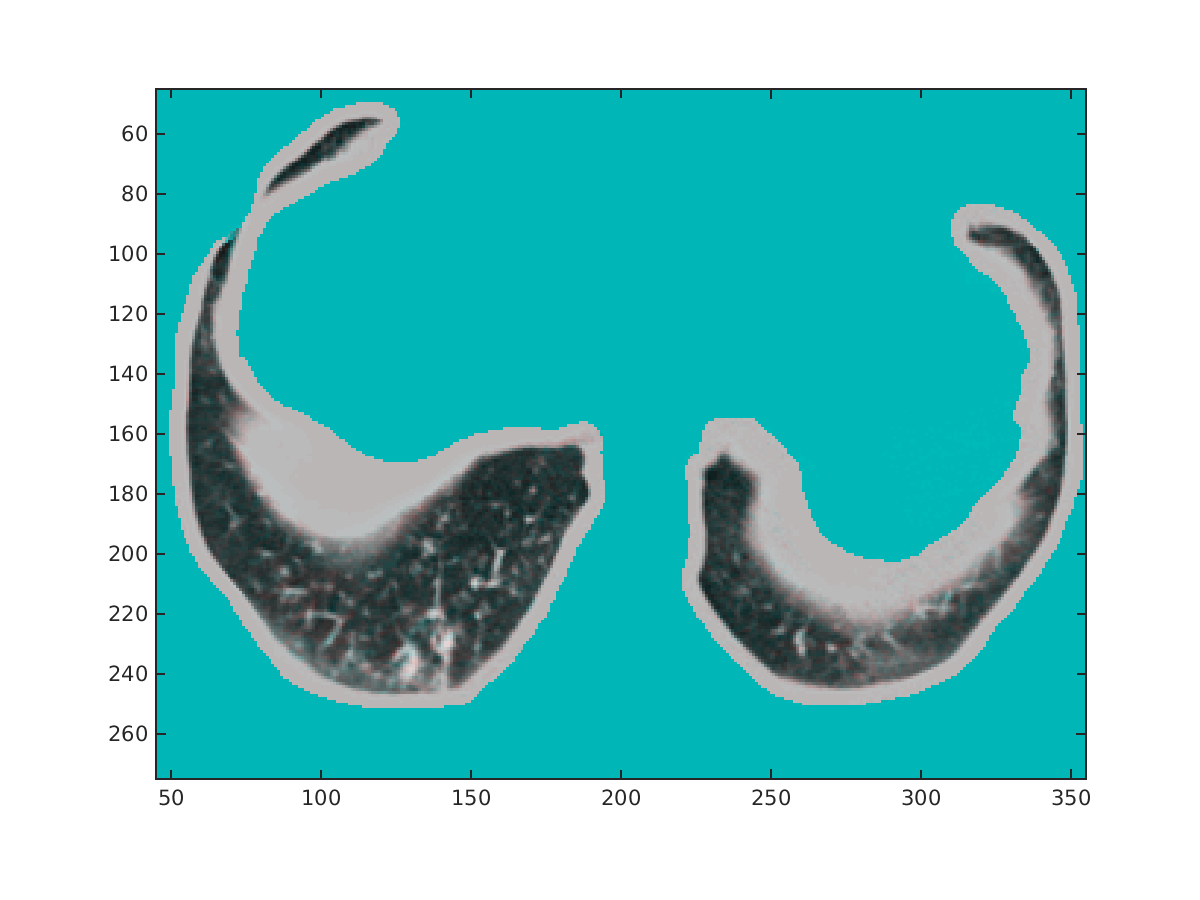
\includegraphics[width=\textwidth, trim=20 20 20 20]{figures/reg2/reg5_4_25.png}
	  \caption{Couch 5, volume 4, slice 25}
	  \label{fig:c22}
  \end{subfigure}
%         ~ %add desired spacing between images, e. g. ~, \quad, \qquad, \hfill etc.
    %(or a blank line to force the subfigure onto a new line)
  \begin{subfigure}[b]{0.3\textwidth}
	  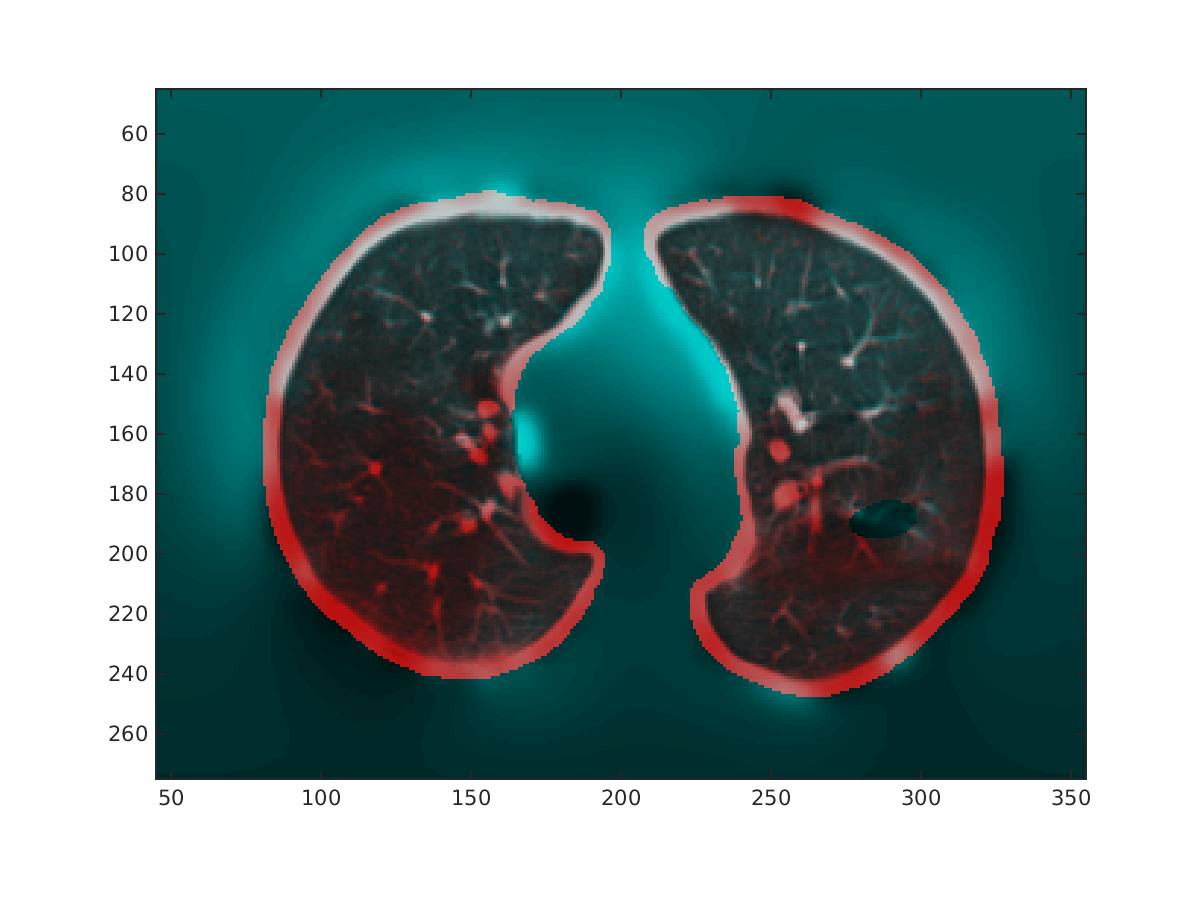
\includegraphics[width=\textwidth, trim=20 20 20 20]{figures/reg2/reg1_6_76.png}
	  \caption{Couch 1, volume 6, slice 76}
	  \label{fig:c23}
  \end{subfigure}
  \caption{Registration results at several different slices and volumes for each couch position. For each subfigure, registration 1 and 2 are shown in the upper and lower figures respectively.}
  \label{fig:c1vis}
\end{figure}


Figure \ref{fig:c1vis} shows the registration results for a few representative slices and volumes over all couch positions. Both registrations perform equally well subfigures (\ref{fig:c11} - \ref{fig:c22}), but yielded a bad registration in subfigure \ref{fig:c23}. Similar bad registrations have been observed in the last slice of each volume. The images show us that there is a considerable ammount of respiratory motion across different slices which needs to be modelled. The shape of the lung is also dramatically different across different couch positions, reaching a concave shape at couch 5. Nevertheless, the segmentation and registration worked fine even for these slices.

\subsection*{Task 2 \& 3 - Fitting the models}

\begin{figure}[H]
  \centering
  \hspace*{-2em}
  \begin{subfigure}[b]{0.33\textwidth}
    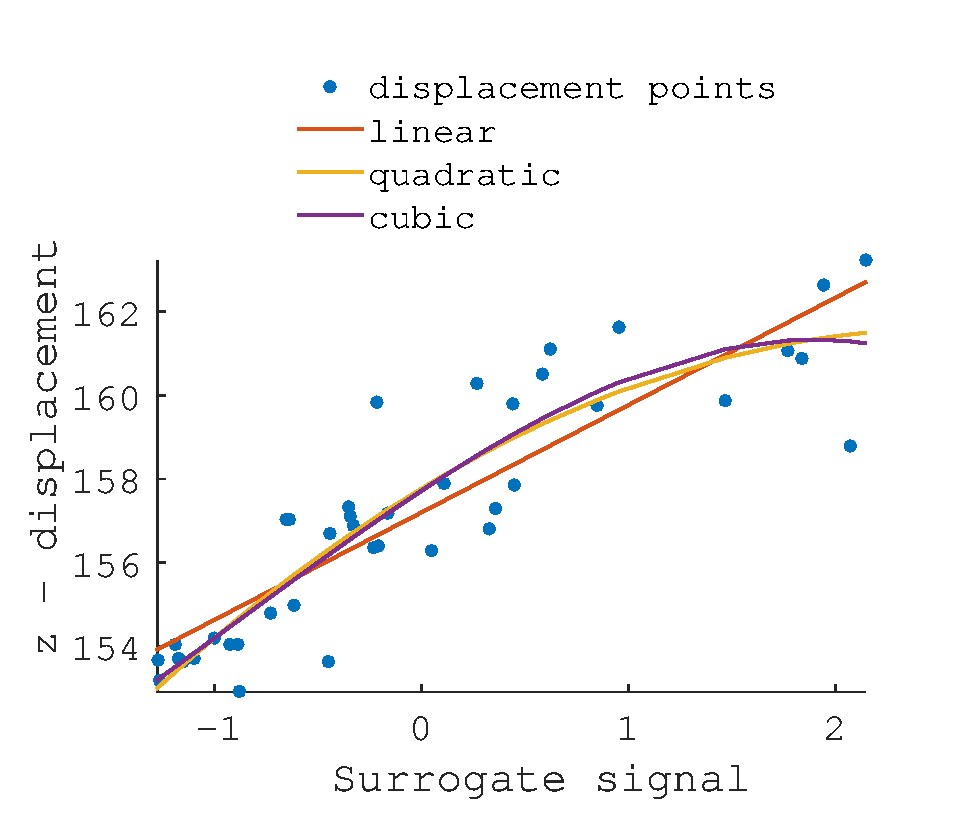
\includegraphics[width=\textwidth]{figures/task2/fit_round1_couch1.eps}
  \end{subfigure}%
    ~ %add desired spacing between images, e. g. ~, \quad, \qquad, \hfill etc.
  %(or a blank line to force the subfigure onto a new line)
  \begin{subfigure}[b]{0.33\textwidth}
    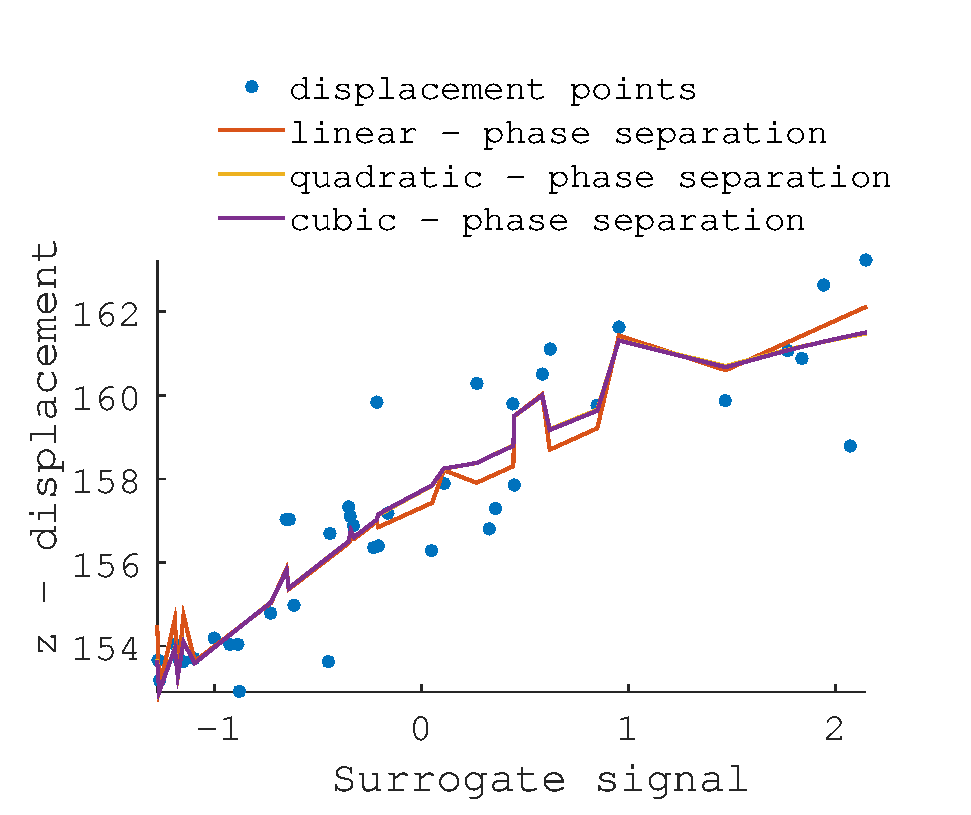
\includegraphics[width=\textwidth]{figures/task2/fit_round2_couch1.eps}
  \end{subfigure}
    ~ %add desired spacing between images, e. g. ~, \quad, \qquad, \hfill etc.
  %     (or a blank line to force the subfigure onto a new line)
  \begin{subfigure}[b]{0.33\textwidth}
    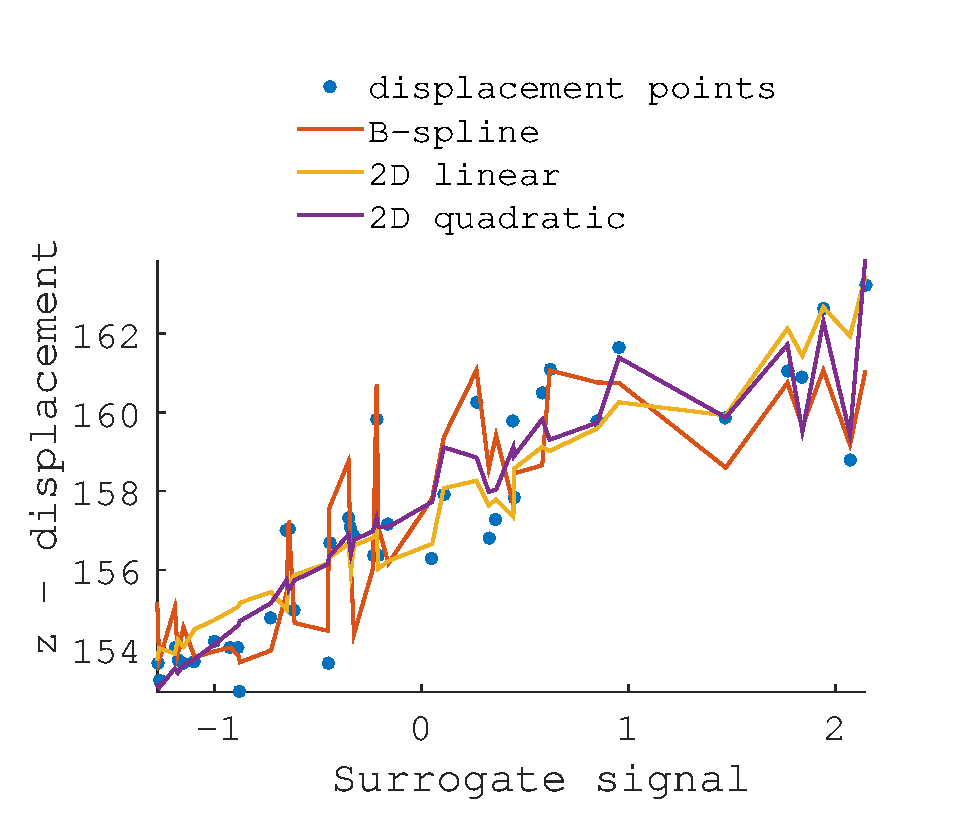
\includegraphics[width=\textwidth]{figures/task2/fit_round3_couch1.eps}
  \end{subfigure}
  (a) Fit for couch position 1, voxel (30,40,33,1,3)
  \vspace*{1em}
  
  \hspace*{-2em}
  \begin{subfigure}[b]{0.33\textwidth}
    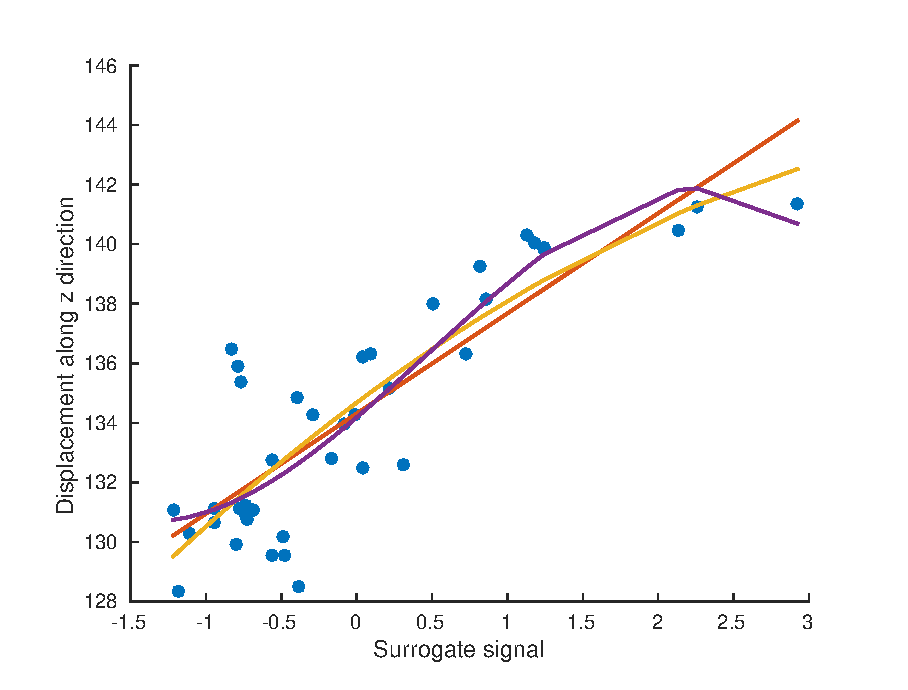
\includegraphics[width=\textwidth, trim=0 0 0 110,clip=true]{figures/task2/fit_round1_couch2.eps}
  \end{subfigure}%
    ~ %add desired spacing between images, e. g. ~, \quad, \qquad, \hfill etc.
%(or a blank line to force the subfigure onto a new line)
  \begin{subfigure}[b]{0.33\textwidth}
    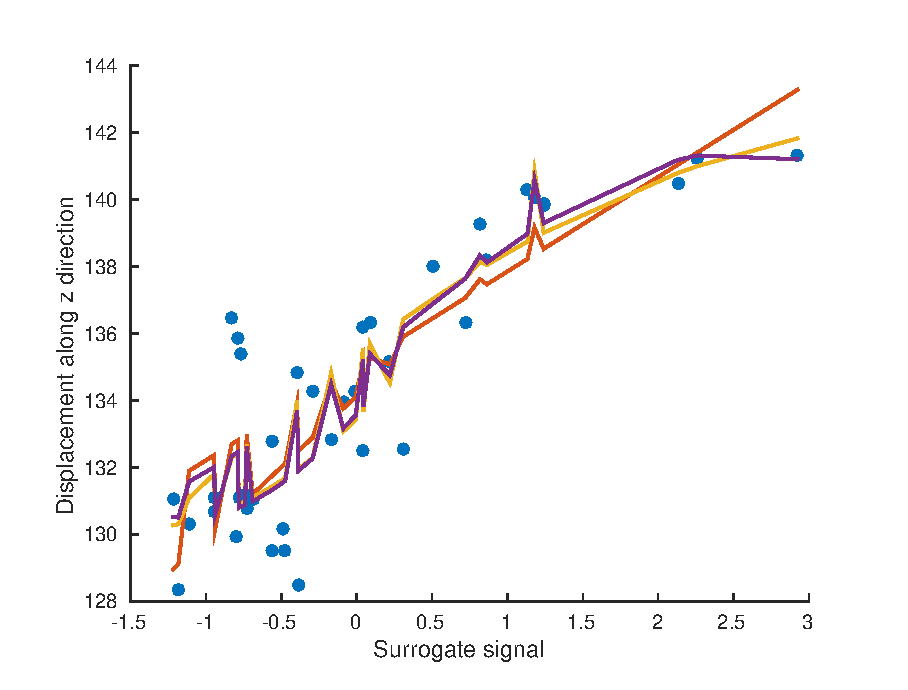
\includegraphics[width=\textwidth, trim=0 0 0 110,clip=true]{figures/task2/fit_round2_couch2.eps}
  \end{subfigure}
    ~ %add desired spacing between images, e. g. ~, \quad, \qquad, \hfill etc.
%     (or a blank line to force the subfigure onto a new line)
  \begin{subfigure}[b]{0.33\textwidth}
    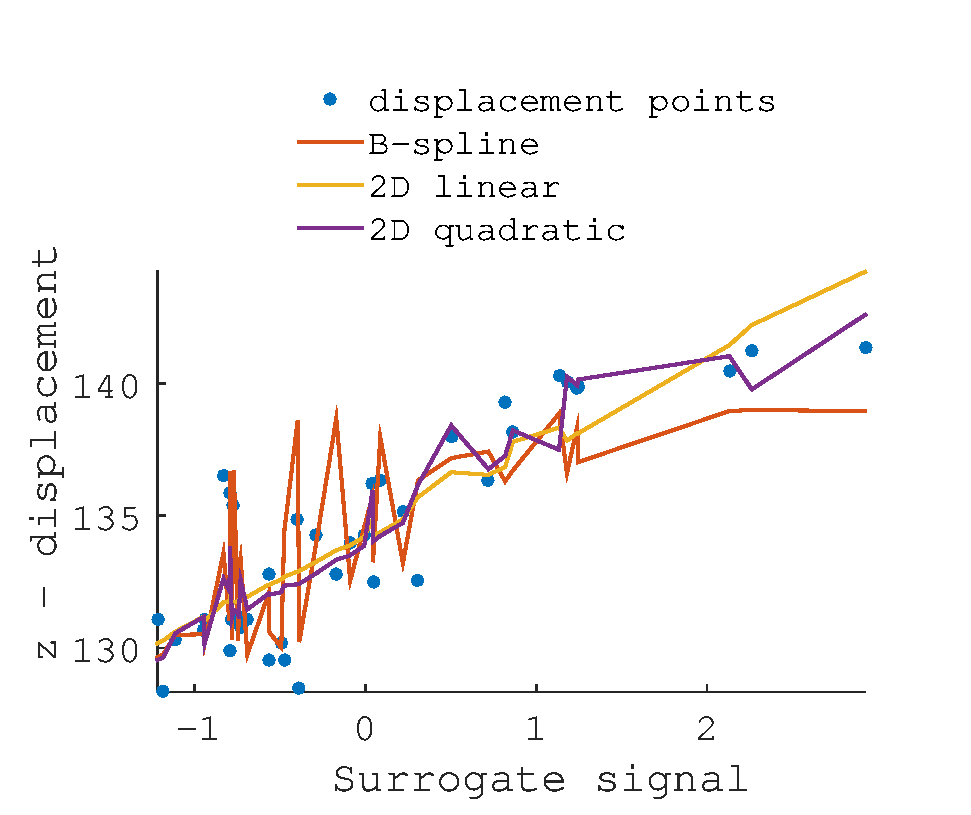
\includegraphics[width=\textwidth, trim=0 0 0 110,clip=true]{figures/task2/fit_round3_couch2.eps}
  \end{subfigure}
  (b) Fit for couch position 2, voxel (30,40,28,1,3)
  \vspace*{1em}
  
    \hspace*{-2em}
  \begin{subfigure}[b]{0.33\textwidth}
    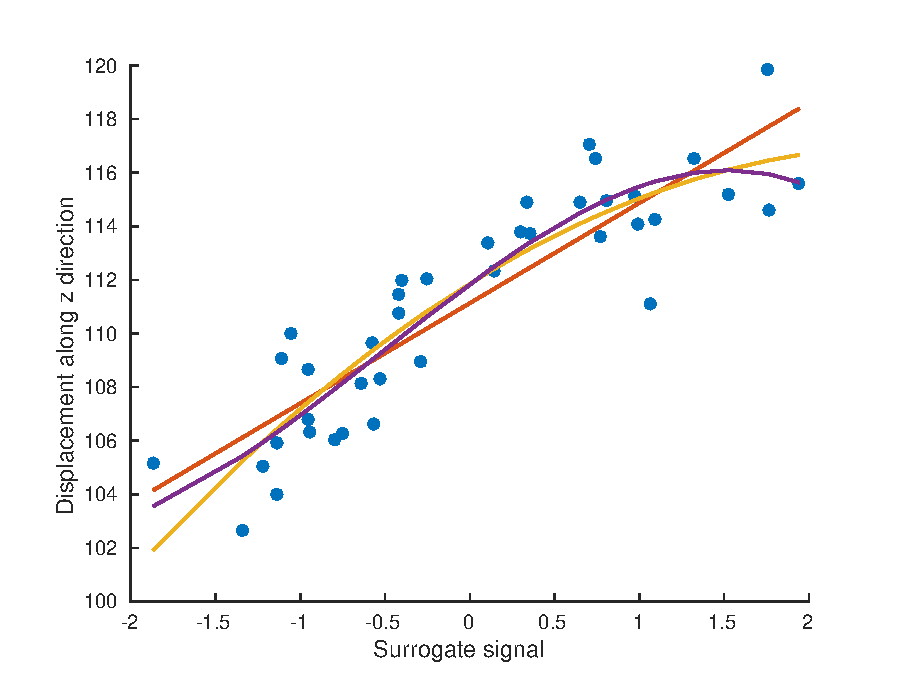
\includegraphics[width=\textwidth, trim=0 0 0 110,clip=true]{figures/task2/fit_round1_couch3.eps}
  \end{subfigure}%
    ~ %add desired spacing between images, e. g. ~, \quad, \qquad, \hfill etc.
%(or a blank line to force the subfigure onto a new line)
  \begin{subfigure}[b]{0.33\textwidth}
    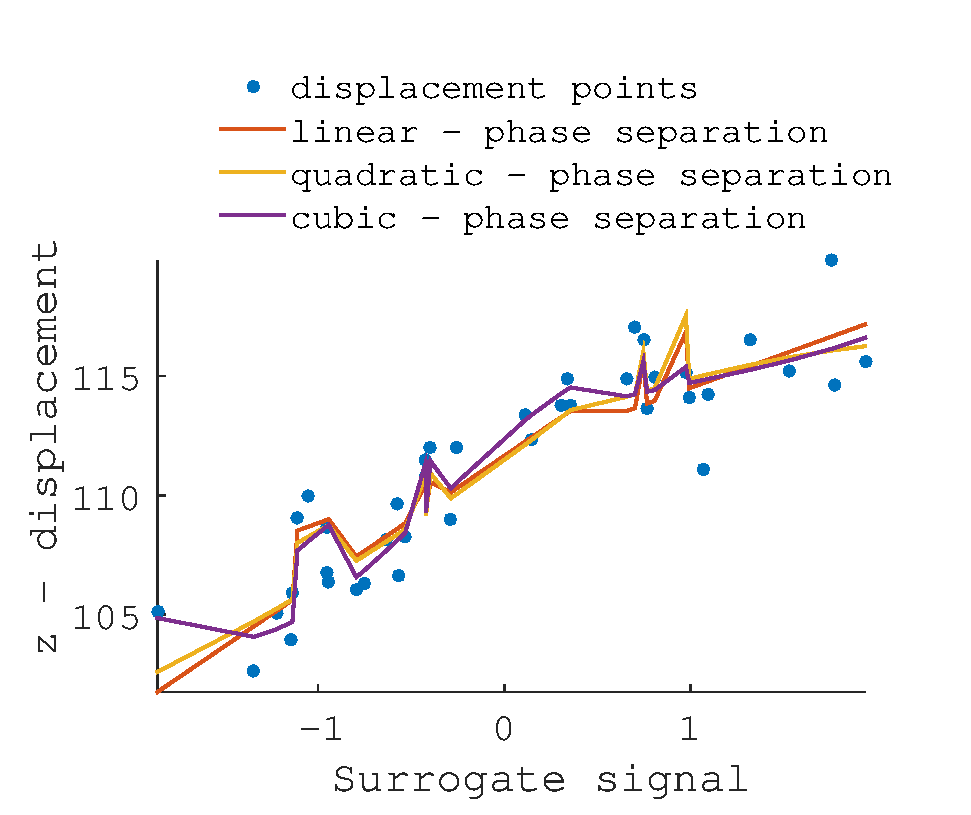
\includegraphics[width=\textwidth, trim=0 0 0 110,clip=true]{figures/task2/fit_round2_couch3.eps}
  \end{subfigure}
    ~ %add desired spacing between images, e. g. ~, \quad, \qquad, \hfill etc.
%     (or a blank line to force the subfigure onto a new line)
  \begin{subfigure}[b]{0.33\textwidth}
    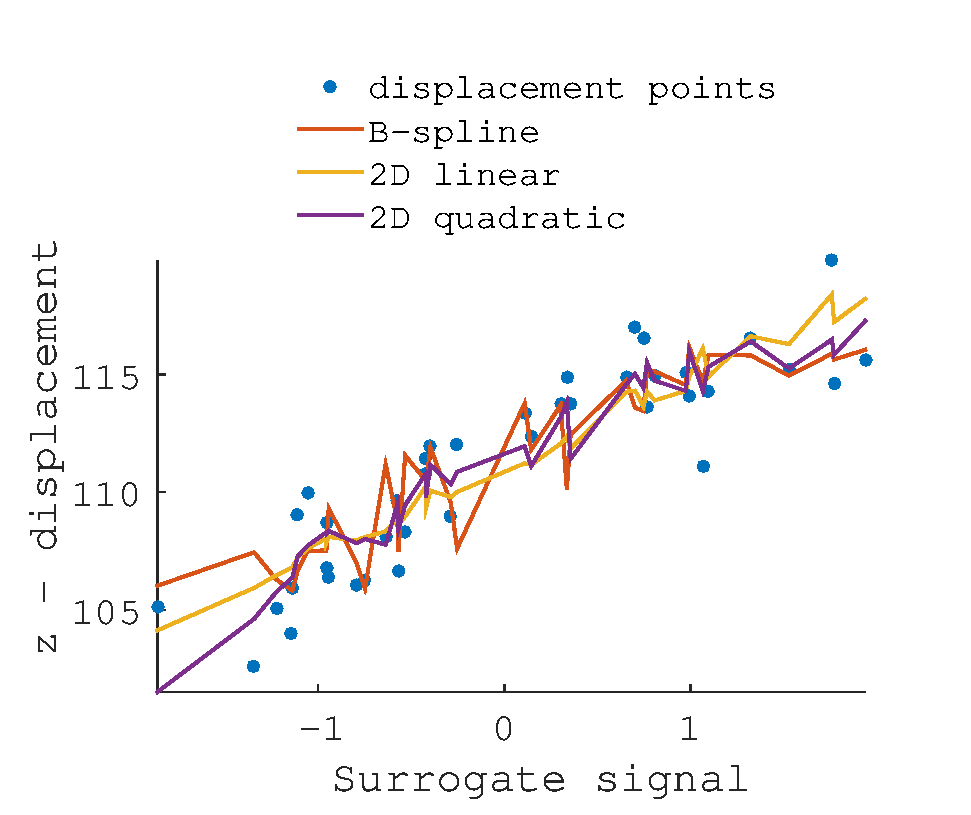
\includegraphics[width=\textwidth, trim=0 0 0 110,clip=true]{figures/task2/fit_round3_couch3.eps}
  \end{subfigure}
  (c) Fit for couch position 3, voxel (30,40,23,1,3)
  \vspace*{1em}
  
    \hspace*{-2em}
  \begin{subfigure}[b]{0.33\textwidth}
    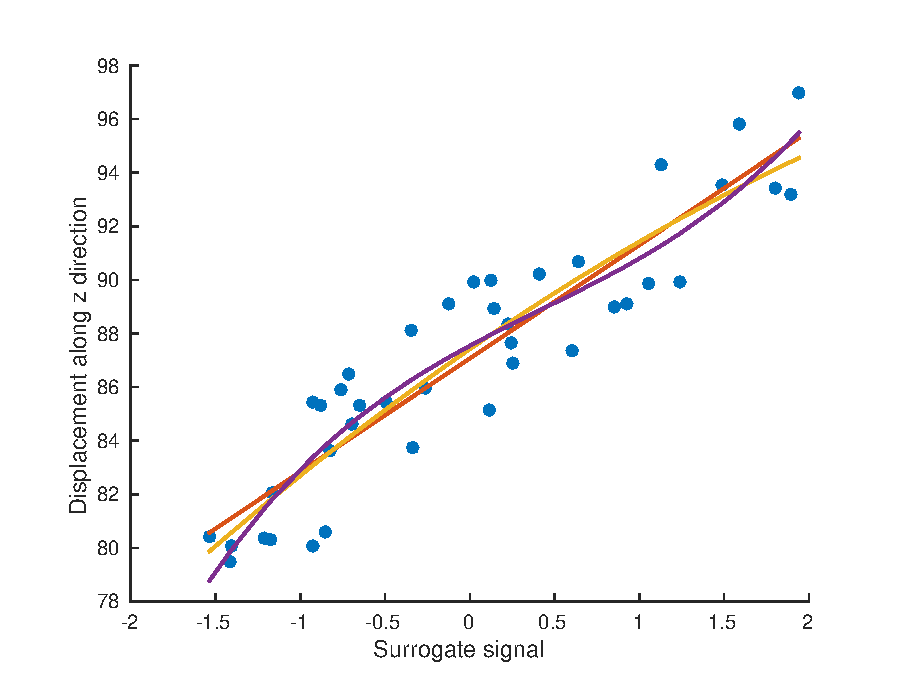
\includegraphics[width=\textwidth, trim=0 0 0 110,clip=true]{figures/task2/fit_round1_couch4.eps}
  \end{subfigure}%
    ~ %add desired spacing between images, e. g. ~, \quad, \qquad, \hfill etc.
%(or a blank line to force the subfigure onto a new line)
  \begin{subfigure}[b]{0.33\textwidth}
    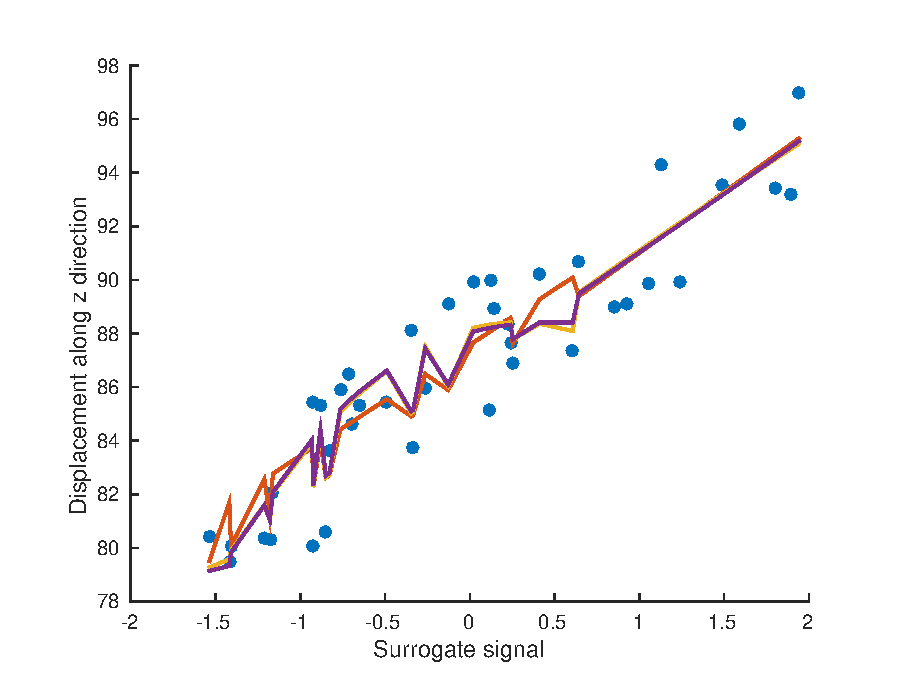
\includegraphics[width=\textwidth, trim=0 0 0 110,clip=true]{figures/task2/fit_round2_couch4.eps}
  \end{subfigure}
    ~ %add desired spacing between images, e. g. ~, \quad, \qquad, \hfill etc.
%     (or a blank line to force the subfigure onto a new line)
  \begin{subfigure}[b]{0.33\textwidth}
    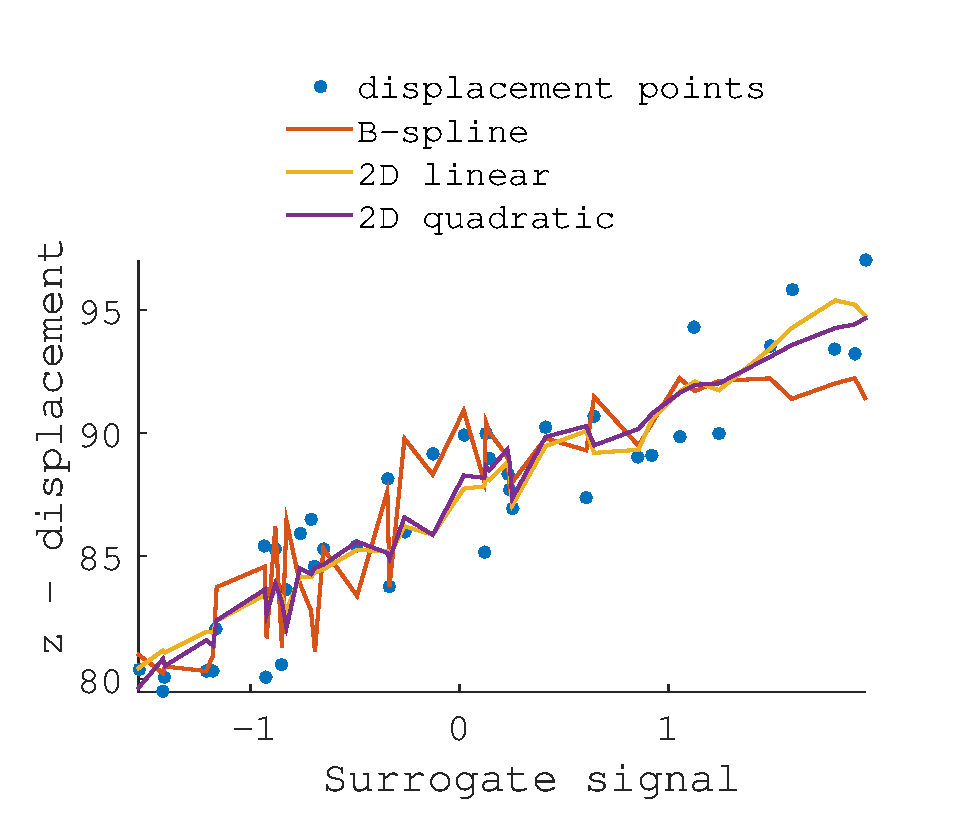
\includegraphics[width=\textwidth, trim=0 0 0 110,clip=true]{figures/task2/fit_round3_couch4.eps}
  \end{subfigure}
   (d) Fit for couch position 4, voxel (30,45,18,1,3)
  \vspace*{1em}

  
    \hspace*{-2em}
  \begin{subfigure}[b]{0.33\textwidth}
    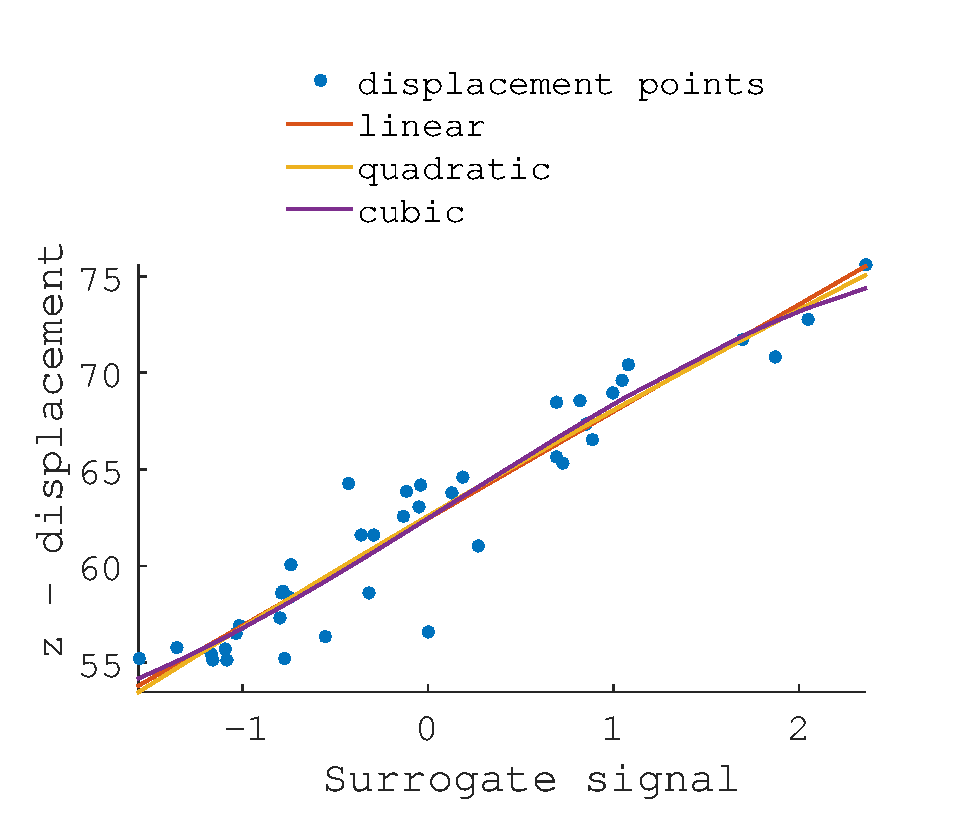
\includegraphics[width=\textwidth, trim=0 0 0 110,clip=true]{figures/task2/fit_round1_couch5.eps}
  \end{subfigure}%
    ~ %add desired spacing between images, e. g. ~, \quad, \qquad, \hfill etc.
%(or a blank line to force the subfigure onto a new line)
  \begin{subfigure}[b]{0.33\textwidth}
    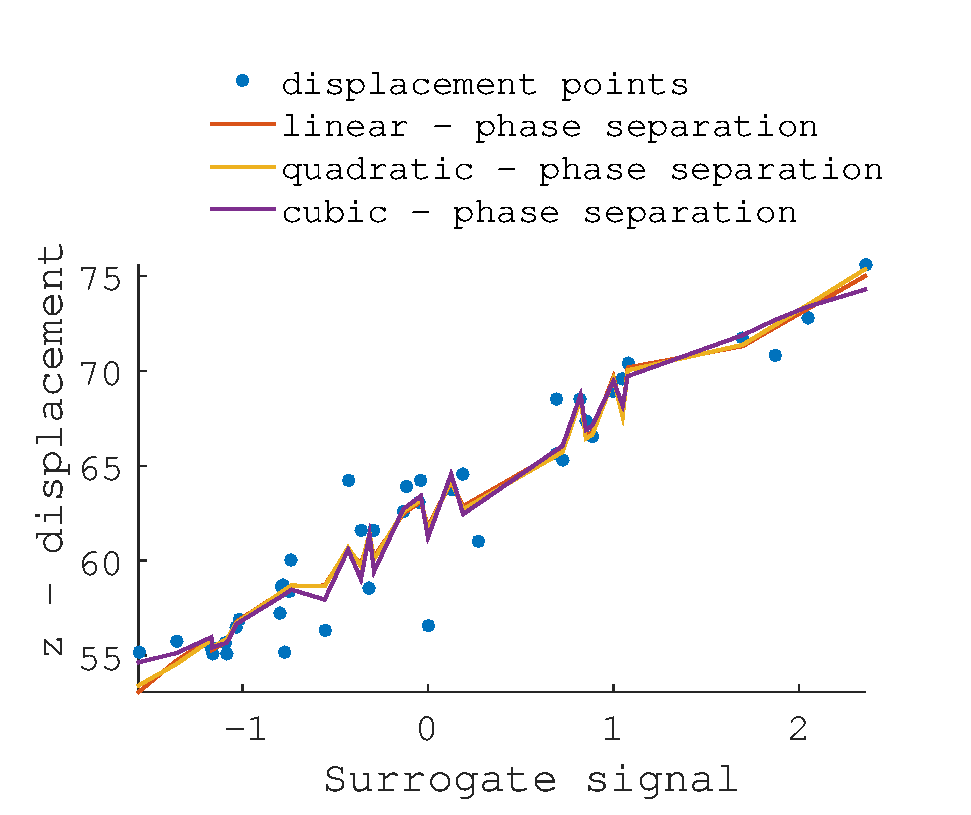
\includegraphics[width=\textwidth, trim=0 0 0 110,clip=true]{figures/task2/fit_round2_couch5.eps}
  \end{subfigure}
    ~ %add desired spacing between images, e. g. ~, \quad, \qquad, \hfill etc.
%     (or a blank line to force the subfigure onto a new line)
  \begin{subfigure}[b]{0.33\textwidth}
    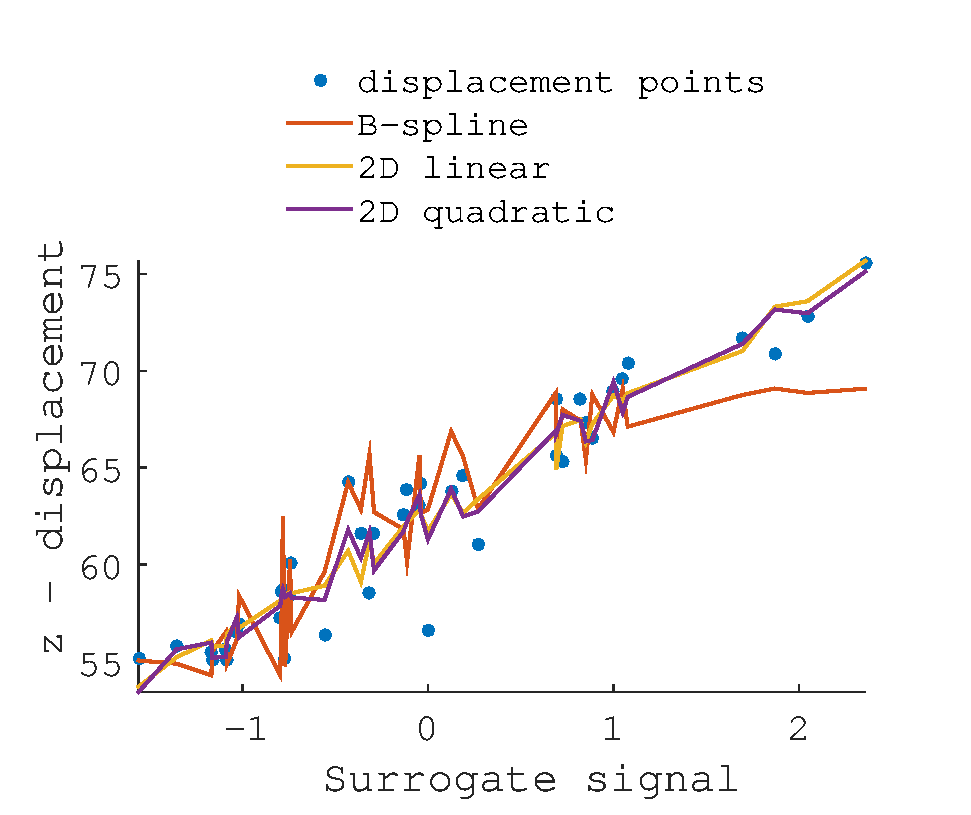
\includegraphics[width=\textwidth, trim=0 0 0 110,clip=true]{figures/task2/fit_round3_couch5.eps}
  \end{subfigure}
  (e) Fit for couch position 5, voxel (30,45,13,1,3)
  \vspace*{1em}

  
  \caption{Fit of 9 different models across 5 voxels each from a different couch position. The first column shows the fit for the three basic models: linear, quadratic and cubic. The second column shows the same models with phase separation, while the last column shows the fit for the B-spline, 2D linear and 2D quadratic models.}
  \label{fig:c2fit}
  
\end{figure}

Figure \ref{fig:c2fit} shows the fit for 9 different models:
\begin{multicols}{3}
\begin{enumerate}
 \item linear
 \item quadratic
 \item cubic
 \item linear - phase separation
 \item quadratic - phase separation
 \item cubic - phase separation
 \item B-spline
 \item 2D linear
 \item 2D quadratic
\end{enumerate}
\end{multicols}





\subsection*{Task 4 - Motion evaluation}

\subsection*{Task 5 - Parameter uncertainty}

\subsection*{Advanced tasks}







\end{document}





















